\documentclass{article}
\usepackage[utf8]{inputenc}
\usepackage{graphicx}
\graphicspath{ {images/} }

\title{FOAR705 - S.Goldie Learning Journal}
\author{Sheriden Goldie}
\date{9th August 2019}

\begin{document}

\maketitle

\section*{Using LaTeX to create a document}

\textbf{Aims:}
\begin{itemize}
    \item familiarise myself with document creation system
    \item create template for learning journal
    \item use template to create entry of process
\end{itemize}

\textbf{Resources:}
\begin{itemize}
    \item Overleaf for LaTeX - Online editor
    \item Overleaf guide - 
    \end{itemize}
\begin{verbatim} https://www.overleaf.com/learn/latex/Learn_LaTeX_in_30_minutes \end{verbatim}



\textbf{Expectations:}
\begin{itemize}
    \item The guide claims to be able to teach me how to cover the basics of LaTeX in 30 minutes
    \item That I will be able to create a document, and replicate this process on my own without the guide
\end{itemize}


\section*{Experience/Errors}

When copying in code from the guide, I duplicated a line which had additional information. The error was highlighted when I tried to recompile the document and I noted that the changes I expected had not been made.
See figure \ref{fig:screenshot1} for detail.

\begin{figure}[ht]
    \centering
    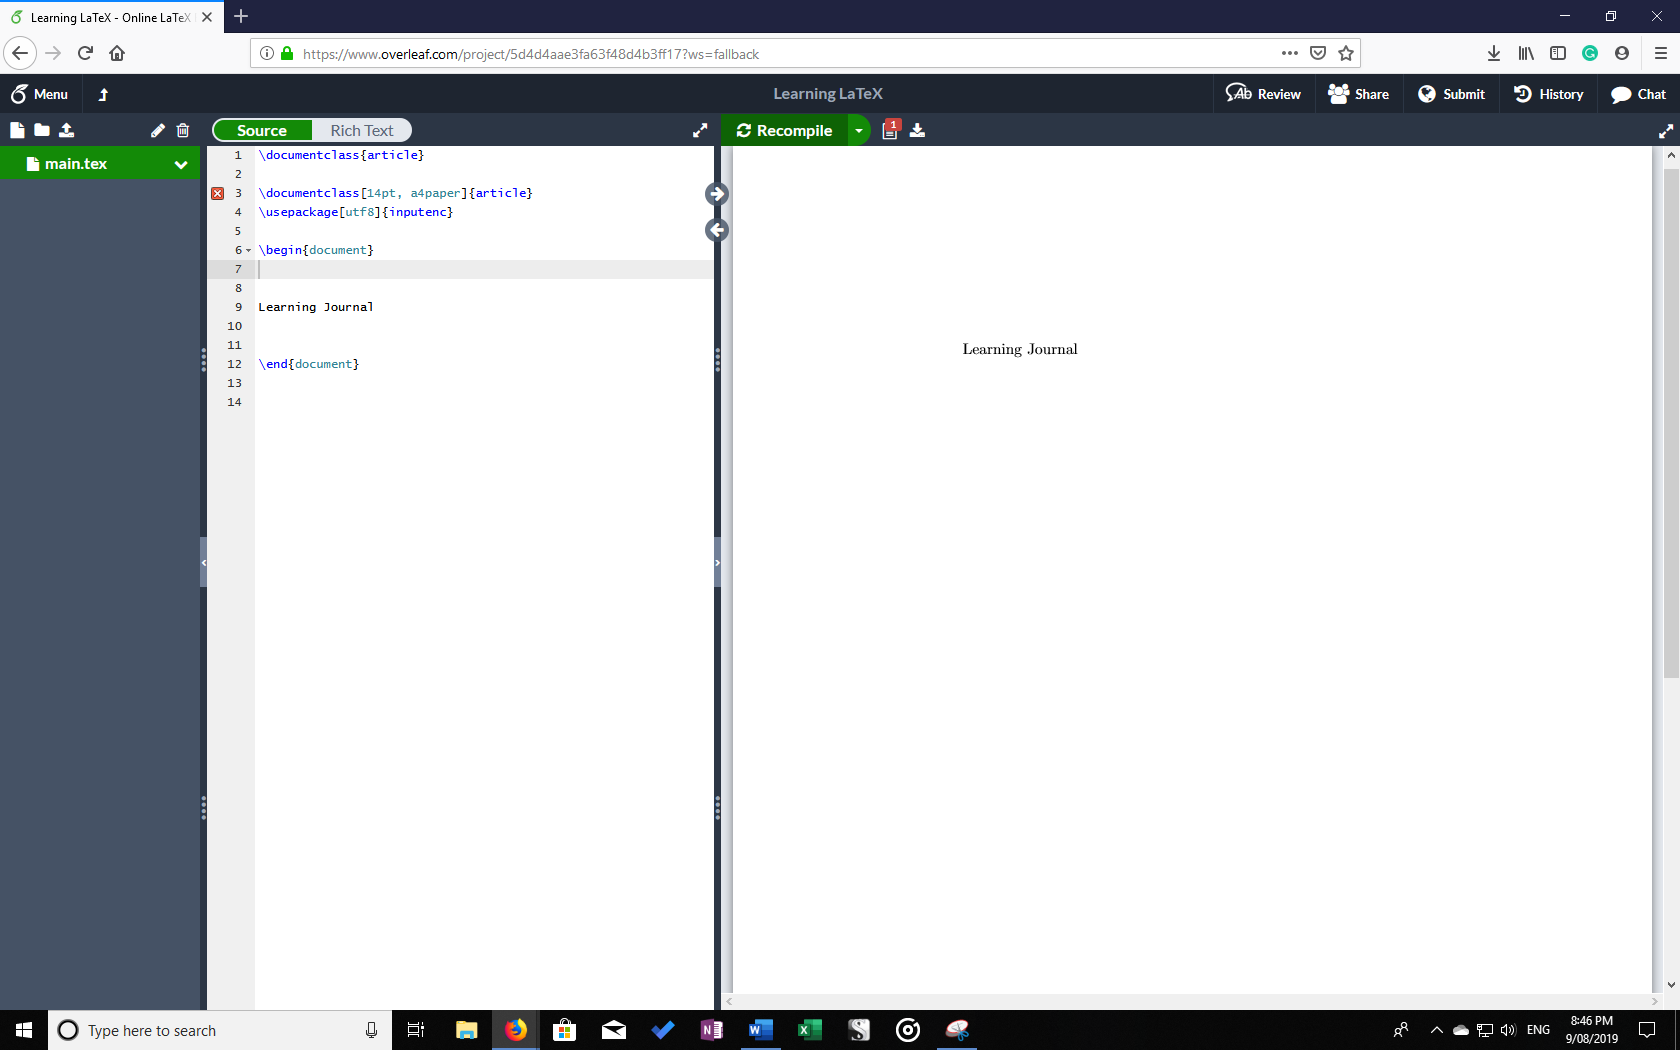
\includegraphics[width=12cm]{Images/Screenshot1.png}
    \caption{My first LaTeX Error}
    \label{fig:screenshot1}
\end{figure}

I removed the first line of code instead of the highlighted one – as I considered that while the highlighted was the second instance but had the more relevant information in it.

I continued following the instructions. See figure \ref{fig:screenshot2} for detail.
I was confused as to why the title/author information wasn’t appearing on the document and spent too long re-reading that section. When I looked at the next section of the guide this was resolved using the "maketitle" code line.

See figure \ref{fig:screenshot3} for error when inserting an image.


\begin{figure}[h]
    \centering
    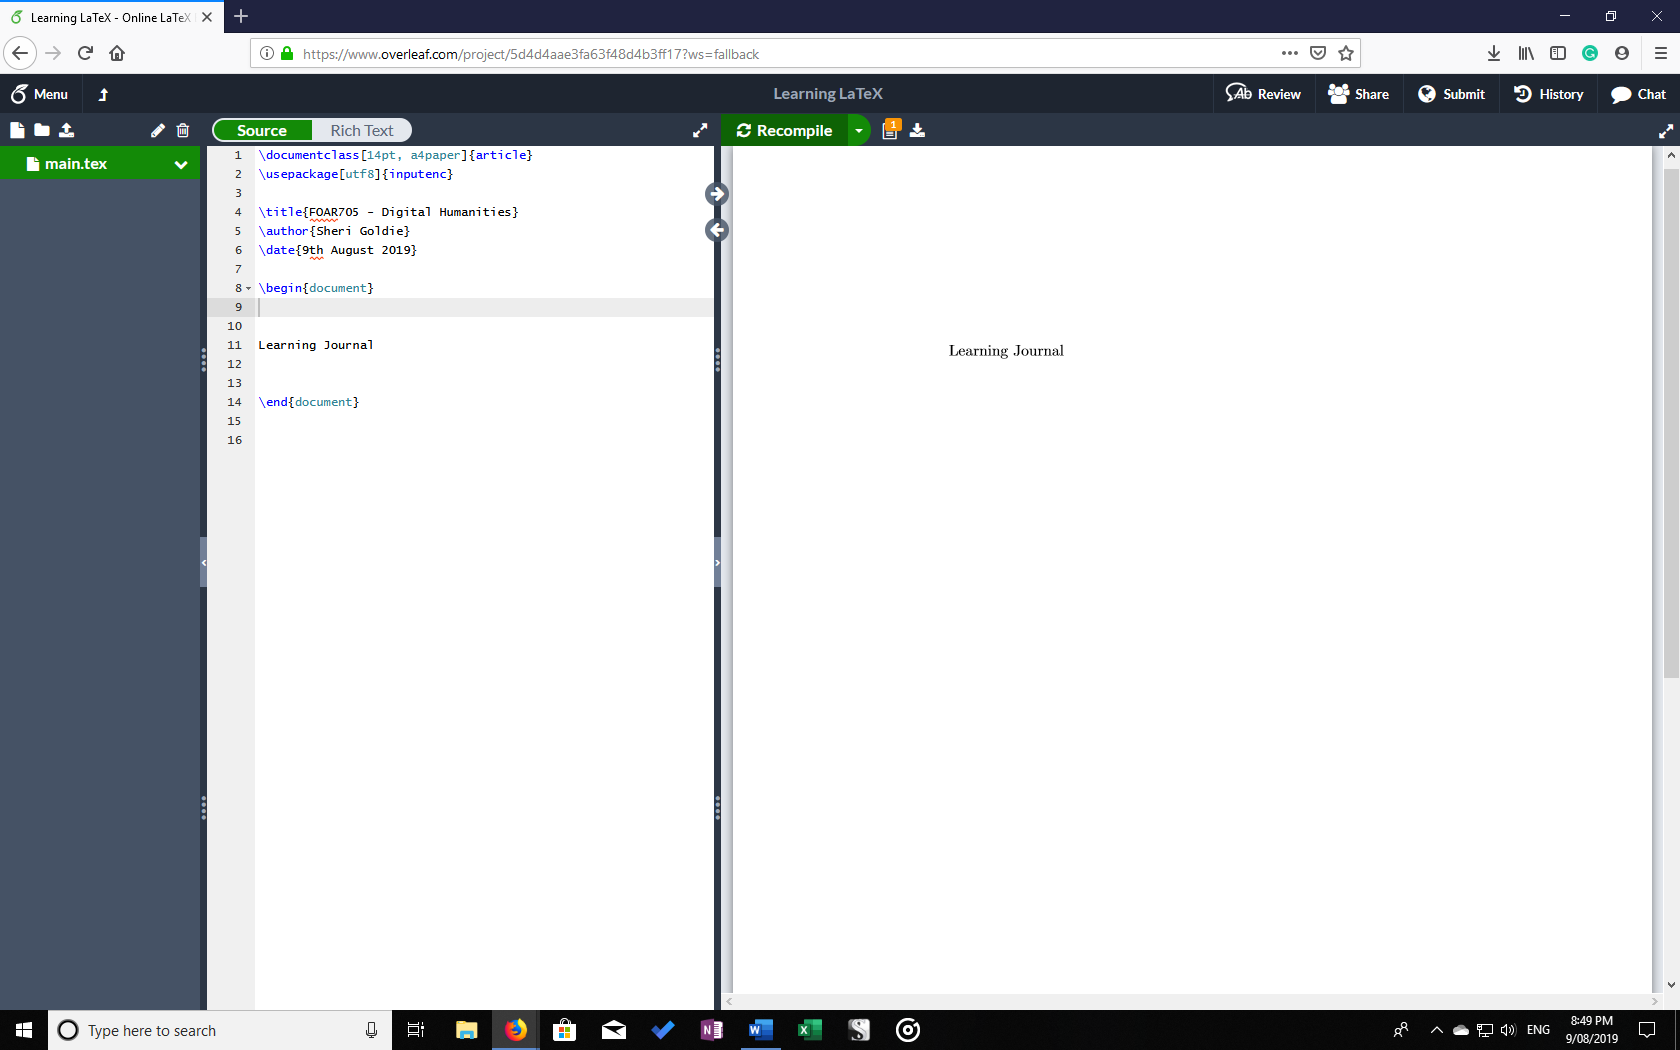
\includegraphics[width=12cm]{Images/Screenshot2.png} 
    \caption{Problem still present}
    \label{fig:screenshot2}
\end{figure}


\begin{figure}[h]
    \centering
    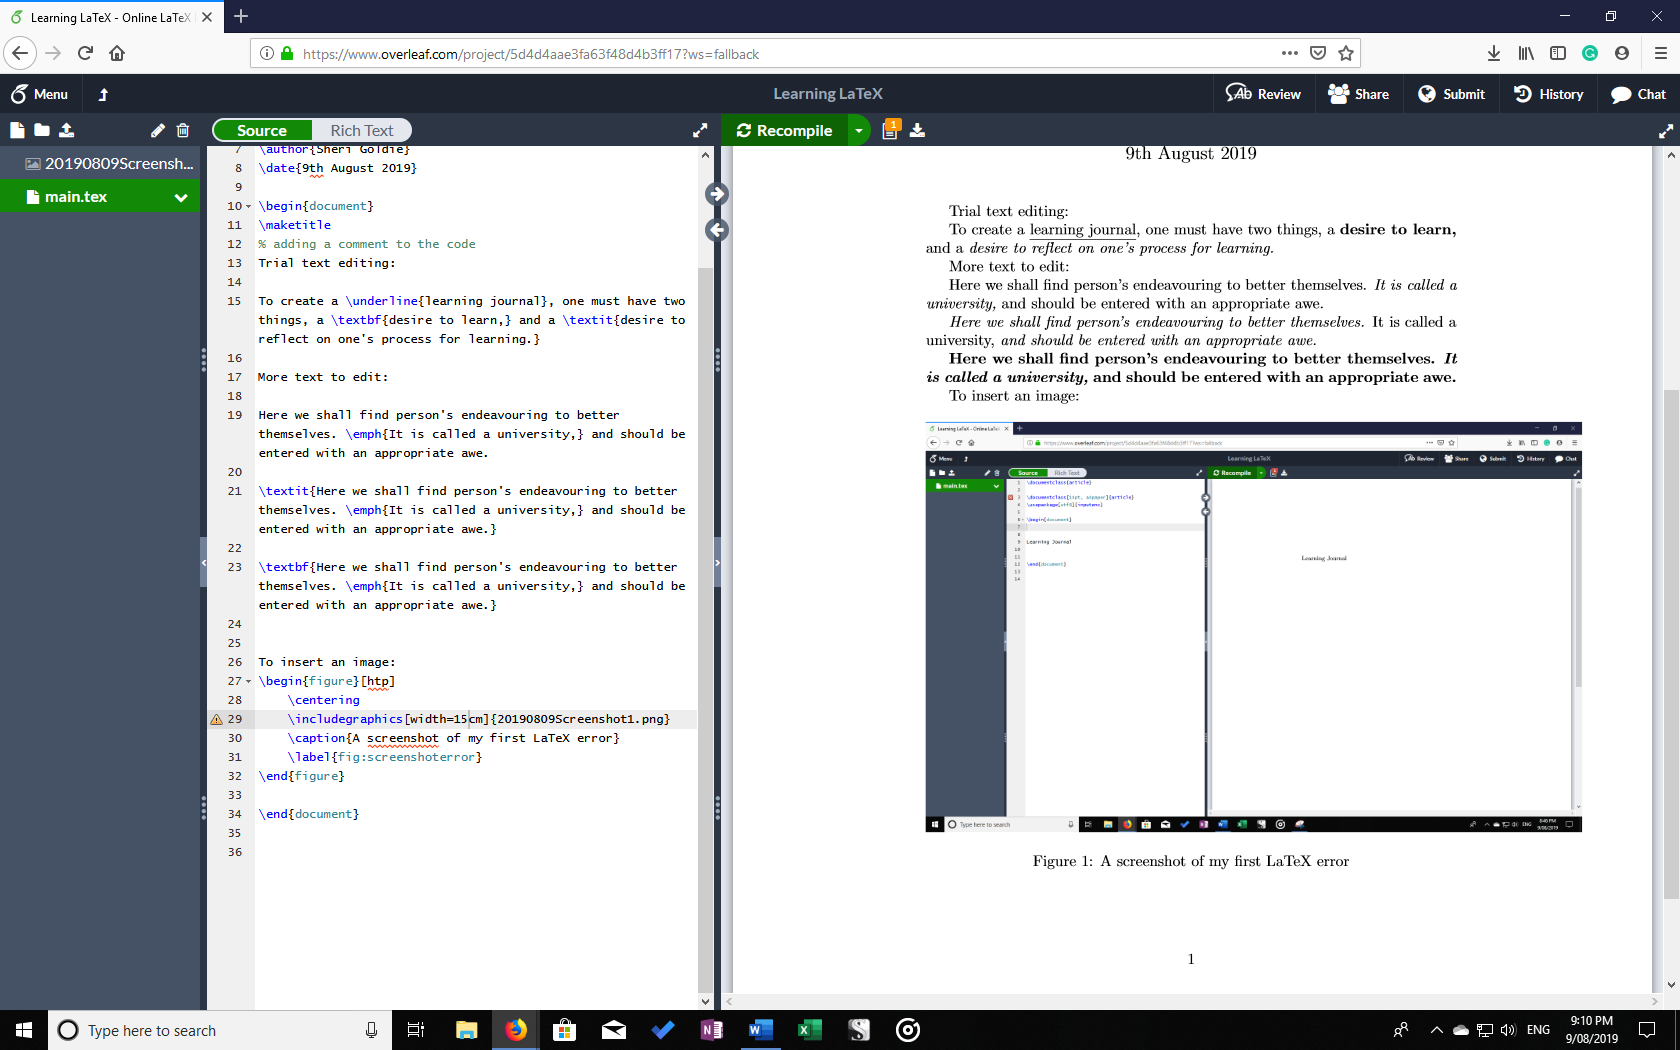
\includegraphics[width=12cm]{Images/Screenshot3.png}
    \caption{Image errors}
    \label{fig:screenshot3}
\end{figure}


\end{document}
